\documentclass[14pt]{extarticle}
\usepackage{calc}
\usepackage{float}
\usepackage{amsmath,amssymb,amsfonts}
\usepackage[T1]{fontenc}
\usepackage{lmodern}
\usepackage{fontspec}
\setmainfont{TeX Gyre Bonum}
\usepackage[english]{babel}
\usepackage[backend=biber,style=authoryear]{biblatex}
\usepackage{array,hhline}
\usepackage{graphicx}
\usepackage[firstpage=true]{background}
\usepackage{csquotes}
\usepackage{verbatim}
\usepackage{glossaries}
\usepackage{makeidx}
\usepackage[expansion=false]{microtype}
\usepackage{xltabular} % The best table package
\usepackage{ragged2e}  % For better text alignment
\usepackage{url}       % Handy for links if needed
\usepackage[colorlinks=false]{hyperref}
\hypersetup{
	linkbordercolor=white, % no box
	pdfborderstyle={/S/U/W 1} % underline style
}

\addbibresource{refs.bib}

% Fix for the specific formatting
\setlength\tabcolsep{1mm}
\setlength{\parskip}{1em}
\renewcommand\arraystretch{1.3}
\backgroundsetup{
	scale=0.9,
	opacity=0.05,
	contents={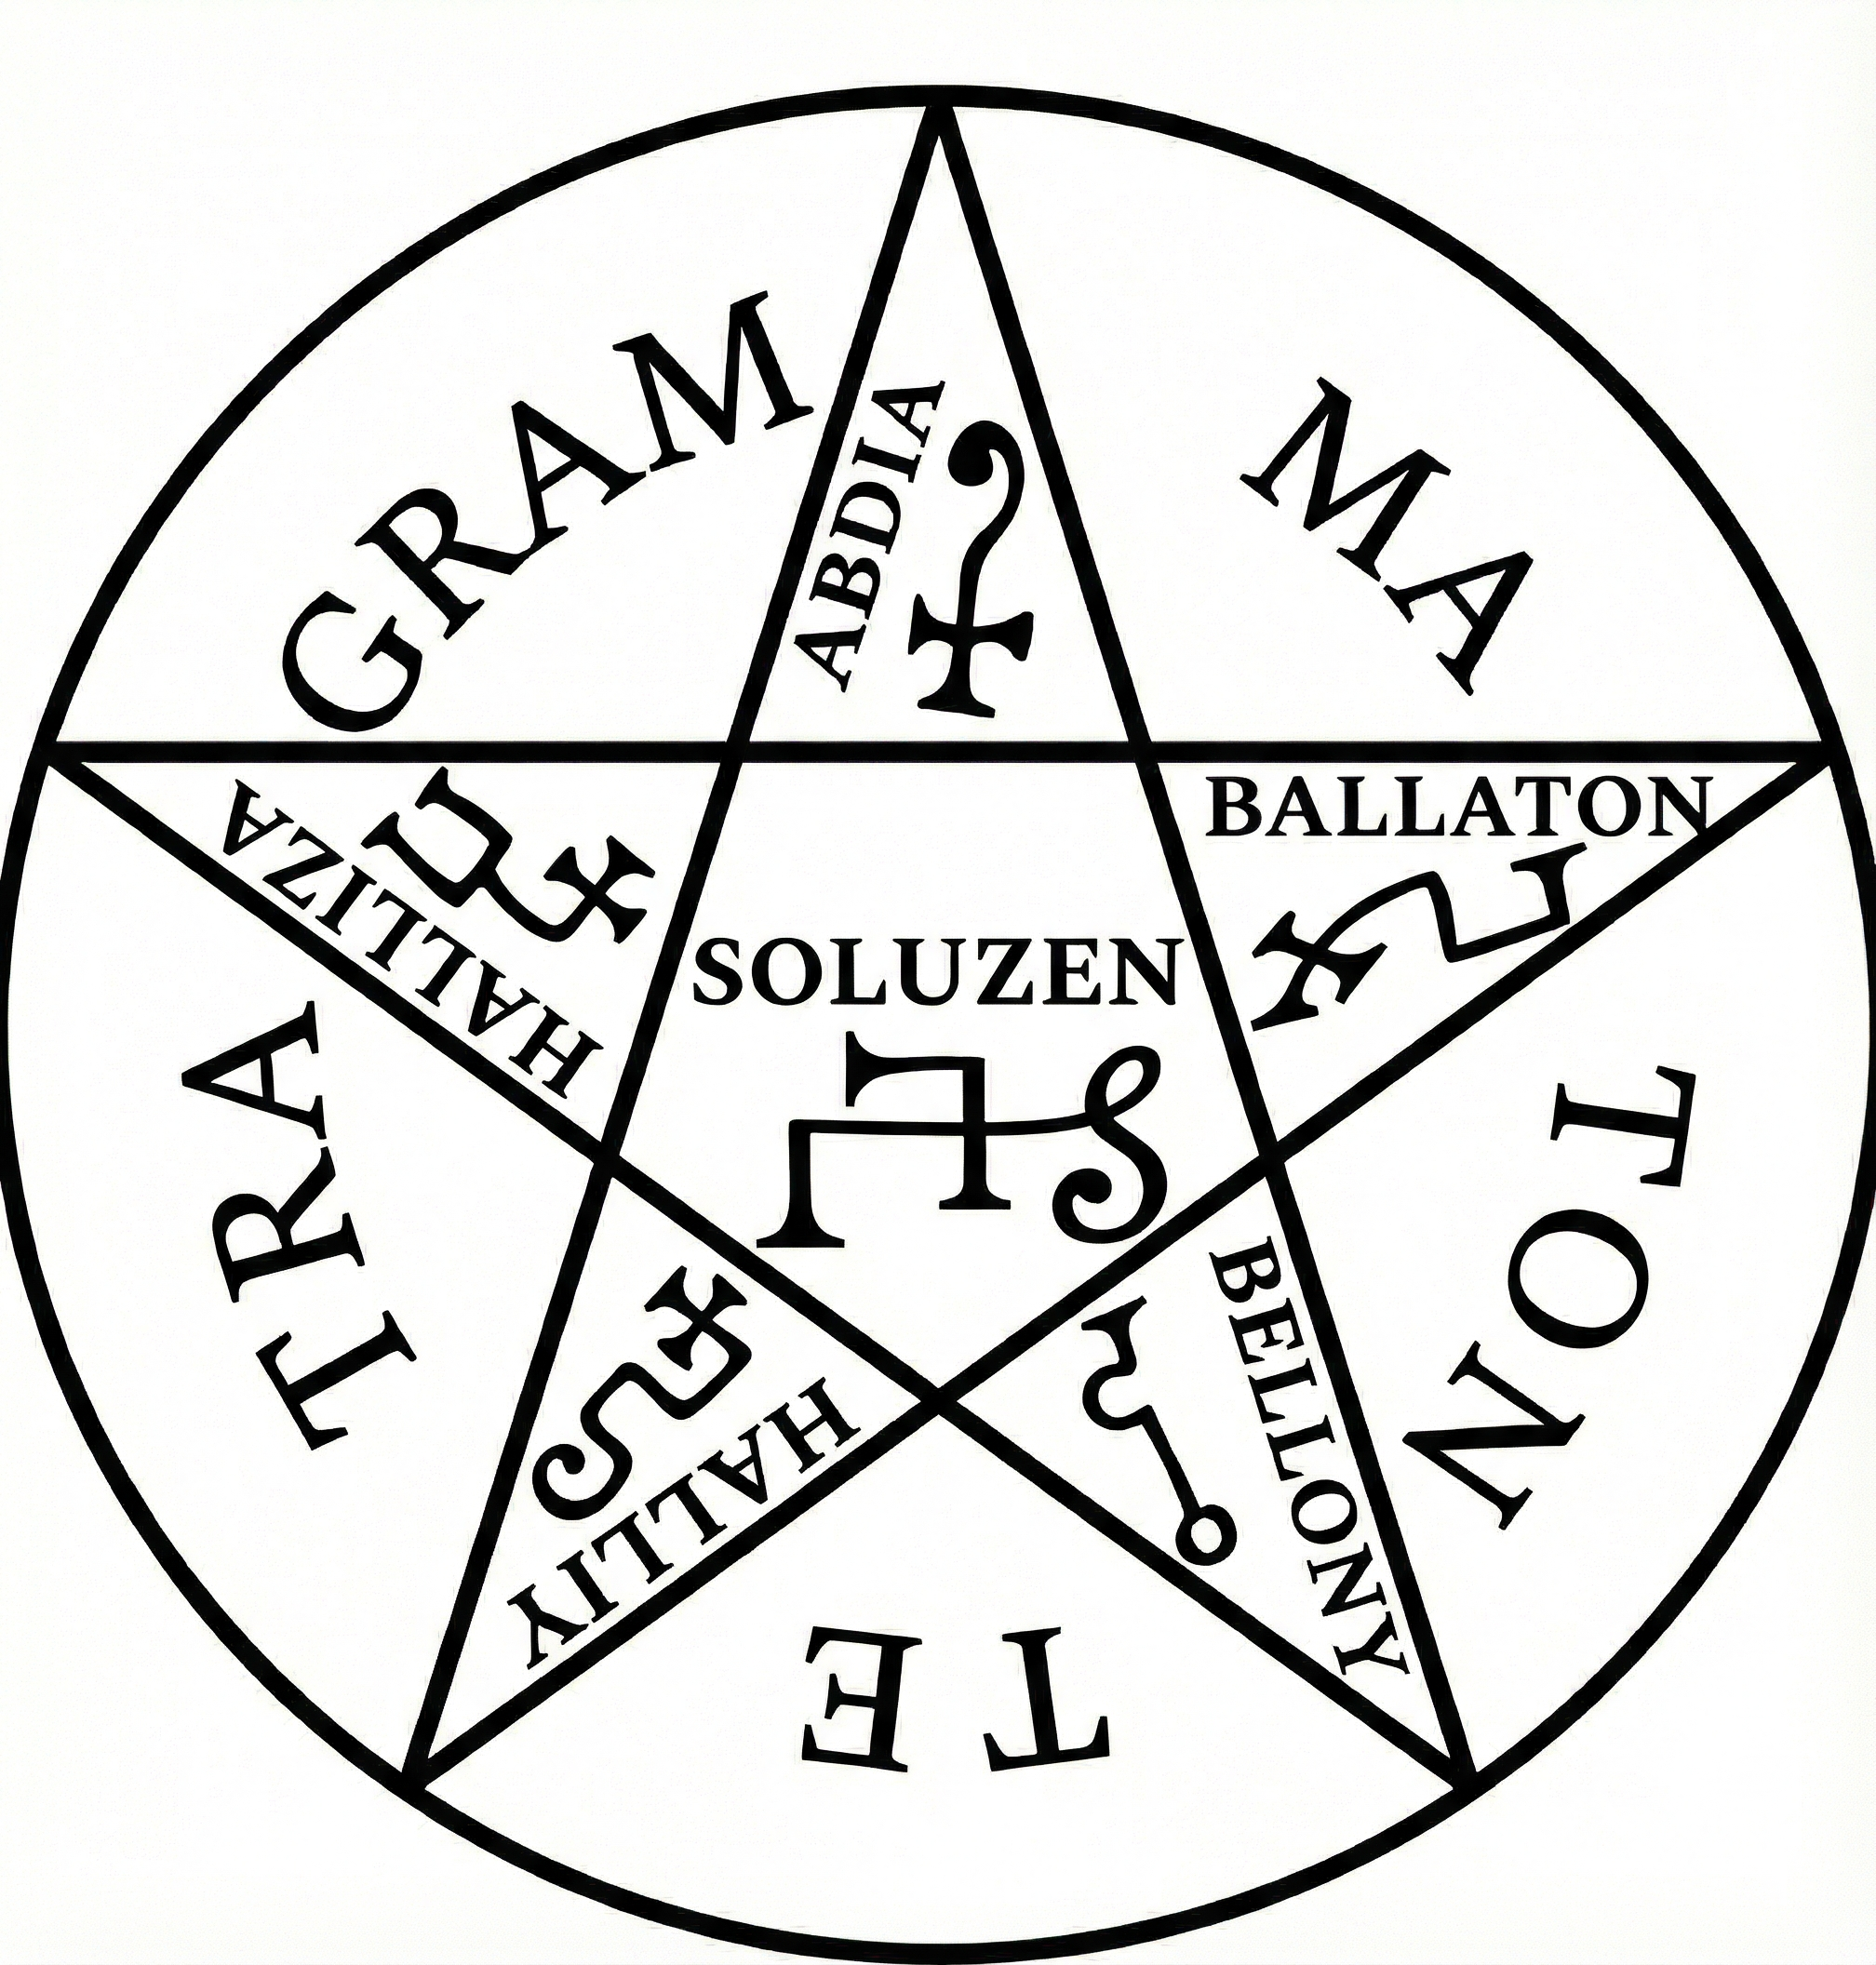
\includegraphics[width=\paperwidth,height=\paperheight,keepaspectratio]{solomon_pentagram.png}}
}

\makeglossary
\makeindex

\hyphenation{TE-TRA-GRAM-MA-TON}

\title{Liber Defensionis}
\author{Michael Stilson}
\date{\today}

\begin{document}
\begin{comment}
	\begin{titlepage}
		\fontfamily{lmodern}\selectfont
		\begin{center}
			\vspace*{\fill}
			\textbf{\Huge LIBER DEFENSIONIS} \\
			\vspace{1.0in}
			{\Large
					A Practical Grimoire of Protection, Entrapment, and Expulsion \\
				\bigskip
					Derived from the Ars Goetia, Babylonian Tradition,
					and Roman Catholic Ritual
			}
			\vspace*{\fill}
		\end{center}
	\end{titlepage}
\end{comment}
	\maketitle
	\thispagestyle{empty}
	\vspace{1.0in}
	\begin{center}
		{\large
			A Practical Grimoire of Protection, Entrapment, and Expulsion \\
			\bigskip
			Derived from the Ars Goetia, Babylonian Tradition,
			and Roman Catholic Ritual
		}
	\end{center}

	\clearpage
	\pagenumbering{roman}
	\tableofcontents
	\clearpage
	\listoffigures
	\clearpage
	\listoftables
	\clearpage

	\pagenumbering{arabic}
\section{INTRODUCTION}
\paragraph{}
Herein is contained the \textit{Liber Defensionis}, a fortress of spirit constructed from three ancient foundations: the \textit{Ars Goetia} (The Lesser Key of Solomon), the Babylonian protective rites of the \textit{Udug-\d{h}ul}, and the exorcistic authority of the \textit{Rituale Romanum}.

While these traditions span millennia and vast theological divides, they share a single, immutable principle: the invocation of Supreme Divine Authority to compel the obedience of lesser spiritual entities.

The Goetic system \cite{mathersgoetia1904} is famously known for the conjuration of spirits, yet hidden within its circles and triangles lies a perfect defensive architecture. The magician was never intended to stand naked before the abyss; the system provides the names of compulsion, the seals of binding, and the geometry of containment. This work inverts the summoner's logic: rather than opening a door to call a spirit \textit{in}, we utilize the keys to lock the spirit \textit{out}.

Complementing this geometry is the primal authority of the Babylonian tradition. Drawing from the \textit{En\={u}ma Eli\v{s}}, we utilize the Fifty Names of Marduk. In the ancient \textit{Marduk’s Address to the Demons}, the \textit{\={a}\v{s}ipu} (exorcist) did not merely pray to the god—he \textit{became} the god, speaking with the voice of the one who slew the chaos-dragon Ti\={a}mat.

Finally, we anchor these ancient forms in the spoken authority of the Roman Catholic tradition, utilizing the \textit{Vade Retro Satana} and the \textit{Prayer to St. Michael}, formulas tempered by centuries of liturgical use against spiritual oppression.

\bigskip

\noindent \textbf{The Structure of the Work:}

\begin{description}
	\item[PART I: Repulsion] \hfill \\
	The establishment of barriers to prevent entry.
	\item[PART II: Entrapment] \hfill \\
	The geometry of containment for localized disturbances.
	\item[PART III: Expulsion] \hfill \\
	The rites of driving out that which has already embedded itself.
	\item[PART IV: The Fifty Names of Marduk] \hfill \\
	The assumption of Babylonian divine authority.
	\item[PART V: Roman Catholic Formulas] \hfill \\
	The traditional litanies of Christian exorcism.
\end{description}
	\clearpage
	\section{REPULSION}
	\hspace{1cm}{\large Preventing Entry and Establishing Defensive Barriers}
	
	\subsection{The Core Logic}
	\paragraph{}
	The Ars Goetia operates on a hierarchy of names and symbols that assert divine authority over all 72 spirits.  The generalized elements are more powerful than individual spirit sigils because they invoke the source of authority rather than targeting an individual entity.  It is like having a master key instead of 72 separate keys.
	
	\subsection{Universal Names of Compulsion}
	These names from the Goetic conjurations work against all spirits of the hierarchy:
	
\begin{flushleft}
	\begin{xltabular}{\textwidth}{|l|X|}
		\hline
		\textbf{Name} & \textbf{Function} \\ \hline
		\endfirsthead
		\hline
		\textbf{Name} & \textbf{Function} \\ \hline
		\endhead
		
		TETRAGRAMMATON & Supreme divine authority (YHVH) \\ \hline
		ADONAI & Lordship and mastery \\ \hline
		AGLA & Protective barrier ("Thou art mighty forever, O Lord") \\ \hline
		PRIMEUMATON & First cause?commands origin \\ \hline
		ANAPHAXETON & Binds the hidden and formless \\ \hline
		EHYEH & "I Am" ? self?existent divine presence \\ \hline
		EL & God (generic, universal) \\ \hline
		ON & Being itself \\ \hline
		\caption{Universal Names of Compulsion}
		
	\end{xltabular}
\end{flushleft}

	\subsection{The Circle of Solomon}
	The original Circle of Solomon serves as the primary protective boundary.  Its key elements include:
	
	Outer Ring:
	
	\begin{itemize}
		\item The names EHYEH, KETHER, METATRON (divine name, sephirah, archangel)
		\item Four pentagrams at cardinal points
		\item Tau crosses (T) representing completion and sealing
	\end{itemize}
	Inner Ring:
	
	\begin{itemize}
		\item TETRAGRAMMATON (YHVH) repeated at quarters
		\item ADONAI inscribed between
	\end{itemize}
	Modification for pure defense: Close all gaps (the original has a {\textquotedblleft}doorway{\textquotedblright} for the spirit
	to perceive the magician). Double the boundary lines.  Add AGLA between each pentagram.
	\begin{figure}[H]
		\centering
		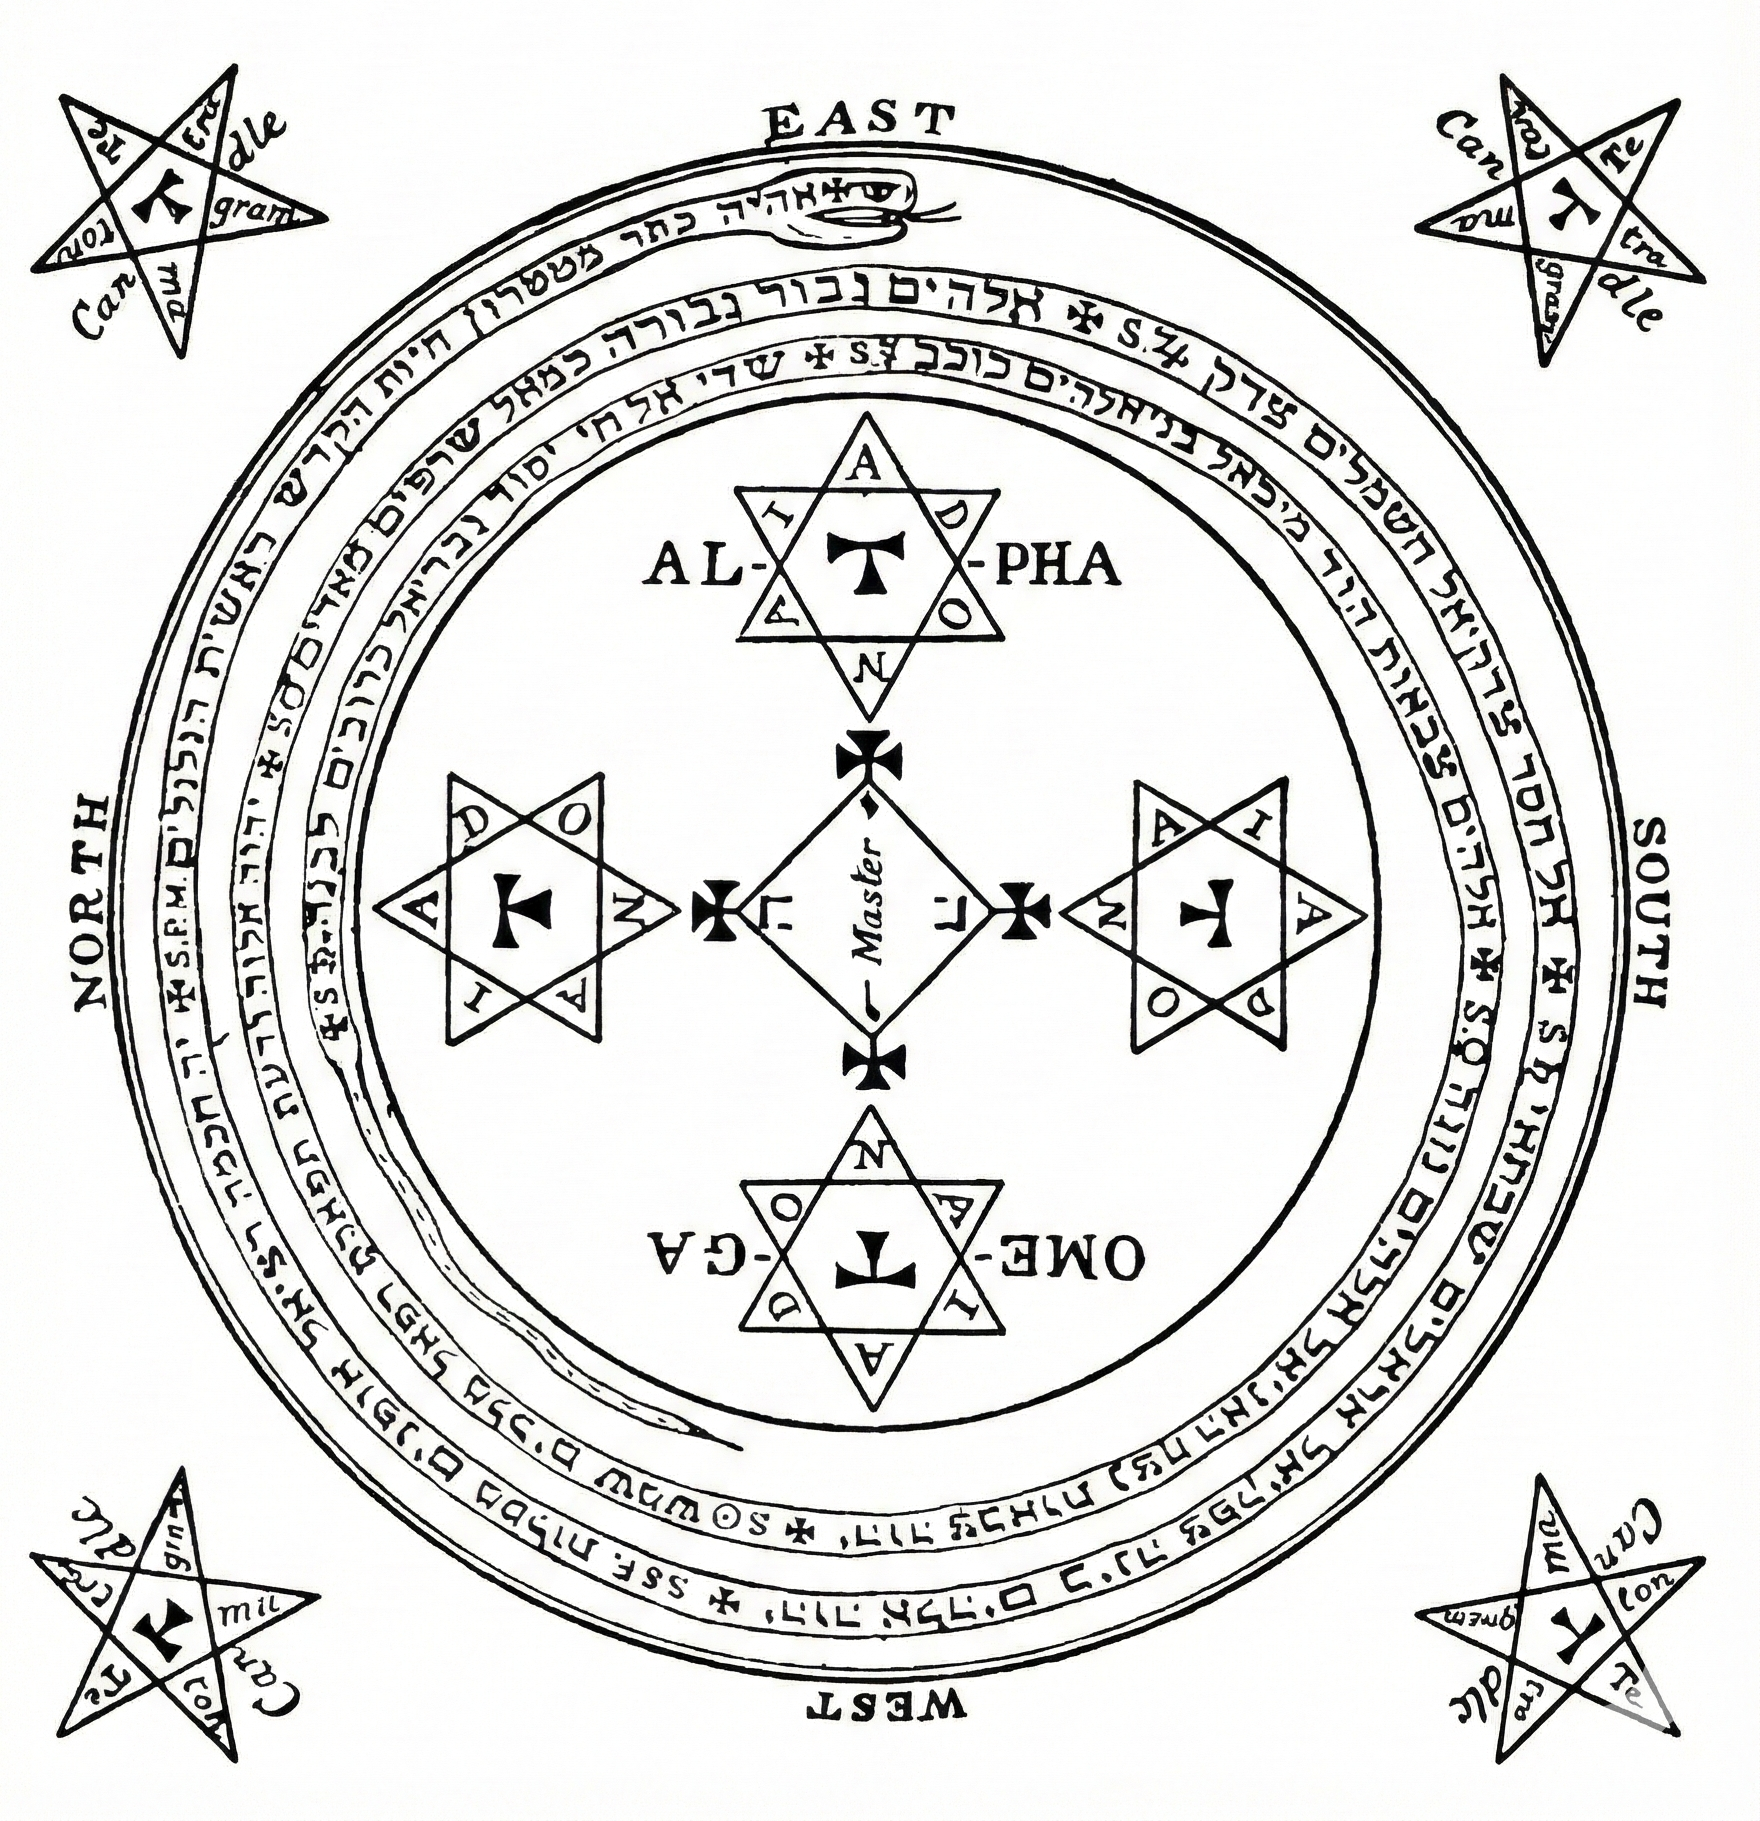
\includegraphics[width=0.3\paperwidth,keepaspectratio]{solomon_circle.png}
		\caption{The Circle of Solomon}
		\label{fig:solomoncircle}
	\end{figure}
	
	\subsection{The Triangle of Art (Repulsion Configuration)}
	For repulsion rather than summoning, the triangle's point faces OUTWARD from the protected space.  The three sides bear:
	\begin{figure}[H]
		\centering
		\includegraphics[width=0.3\paperwidth,keepaspectratio]{solomon_triangle.png}
		\caption{The Triangle of Art}
		\label{fig:solomontriangle}
	\end{figure}
	
	\begin{itemize}
		\item PRIMEUMATON (first moving)
		\item ANAPHAXETON (hidden one)
		\item TETRAGRAMMATON (the Name)
	\end{itemize}
	At the three points, inscribe MI-CHA-EL (Michael)---invoking the archangel who cast down rebellious spirits.  At center, place the Hexagram of Solomon containing no specific name, creating a {\textquotedblleft}blank{\textquotedblright} binding that
	affects any entity.
	\begin{figure}[H]
		\centering
		\includegraphics[width=0.3\paperwidth,keepaspectratio]{solomon_hexagram.png}
		\caption{The Hexagram of Solomon}
		\label{fig:solomonhexagram}
		\cite[39]{mathersgoetia1904}
	\end{figure}
	
	\subsection{The Pentagram of Solomon}
	The most powerful generalized symbol in the system.  Originally worn by the magician for protection.
	\begin{figure}[H]
		\centering
		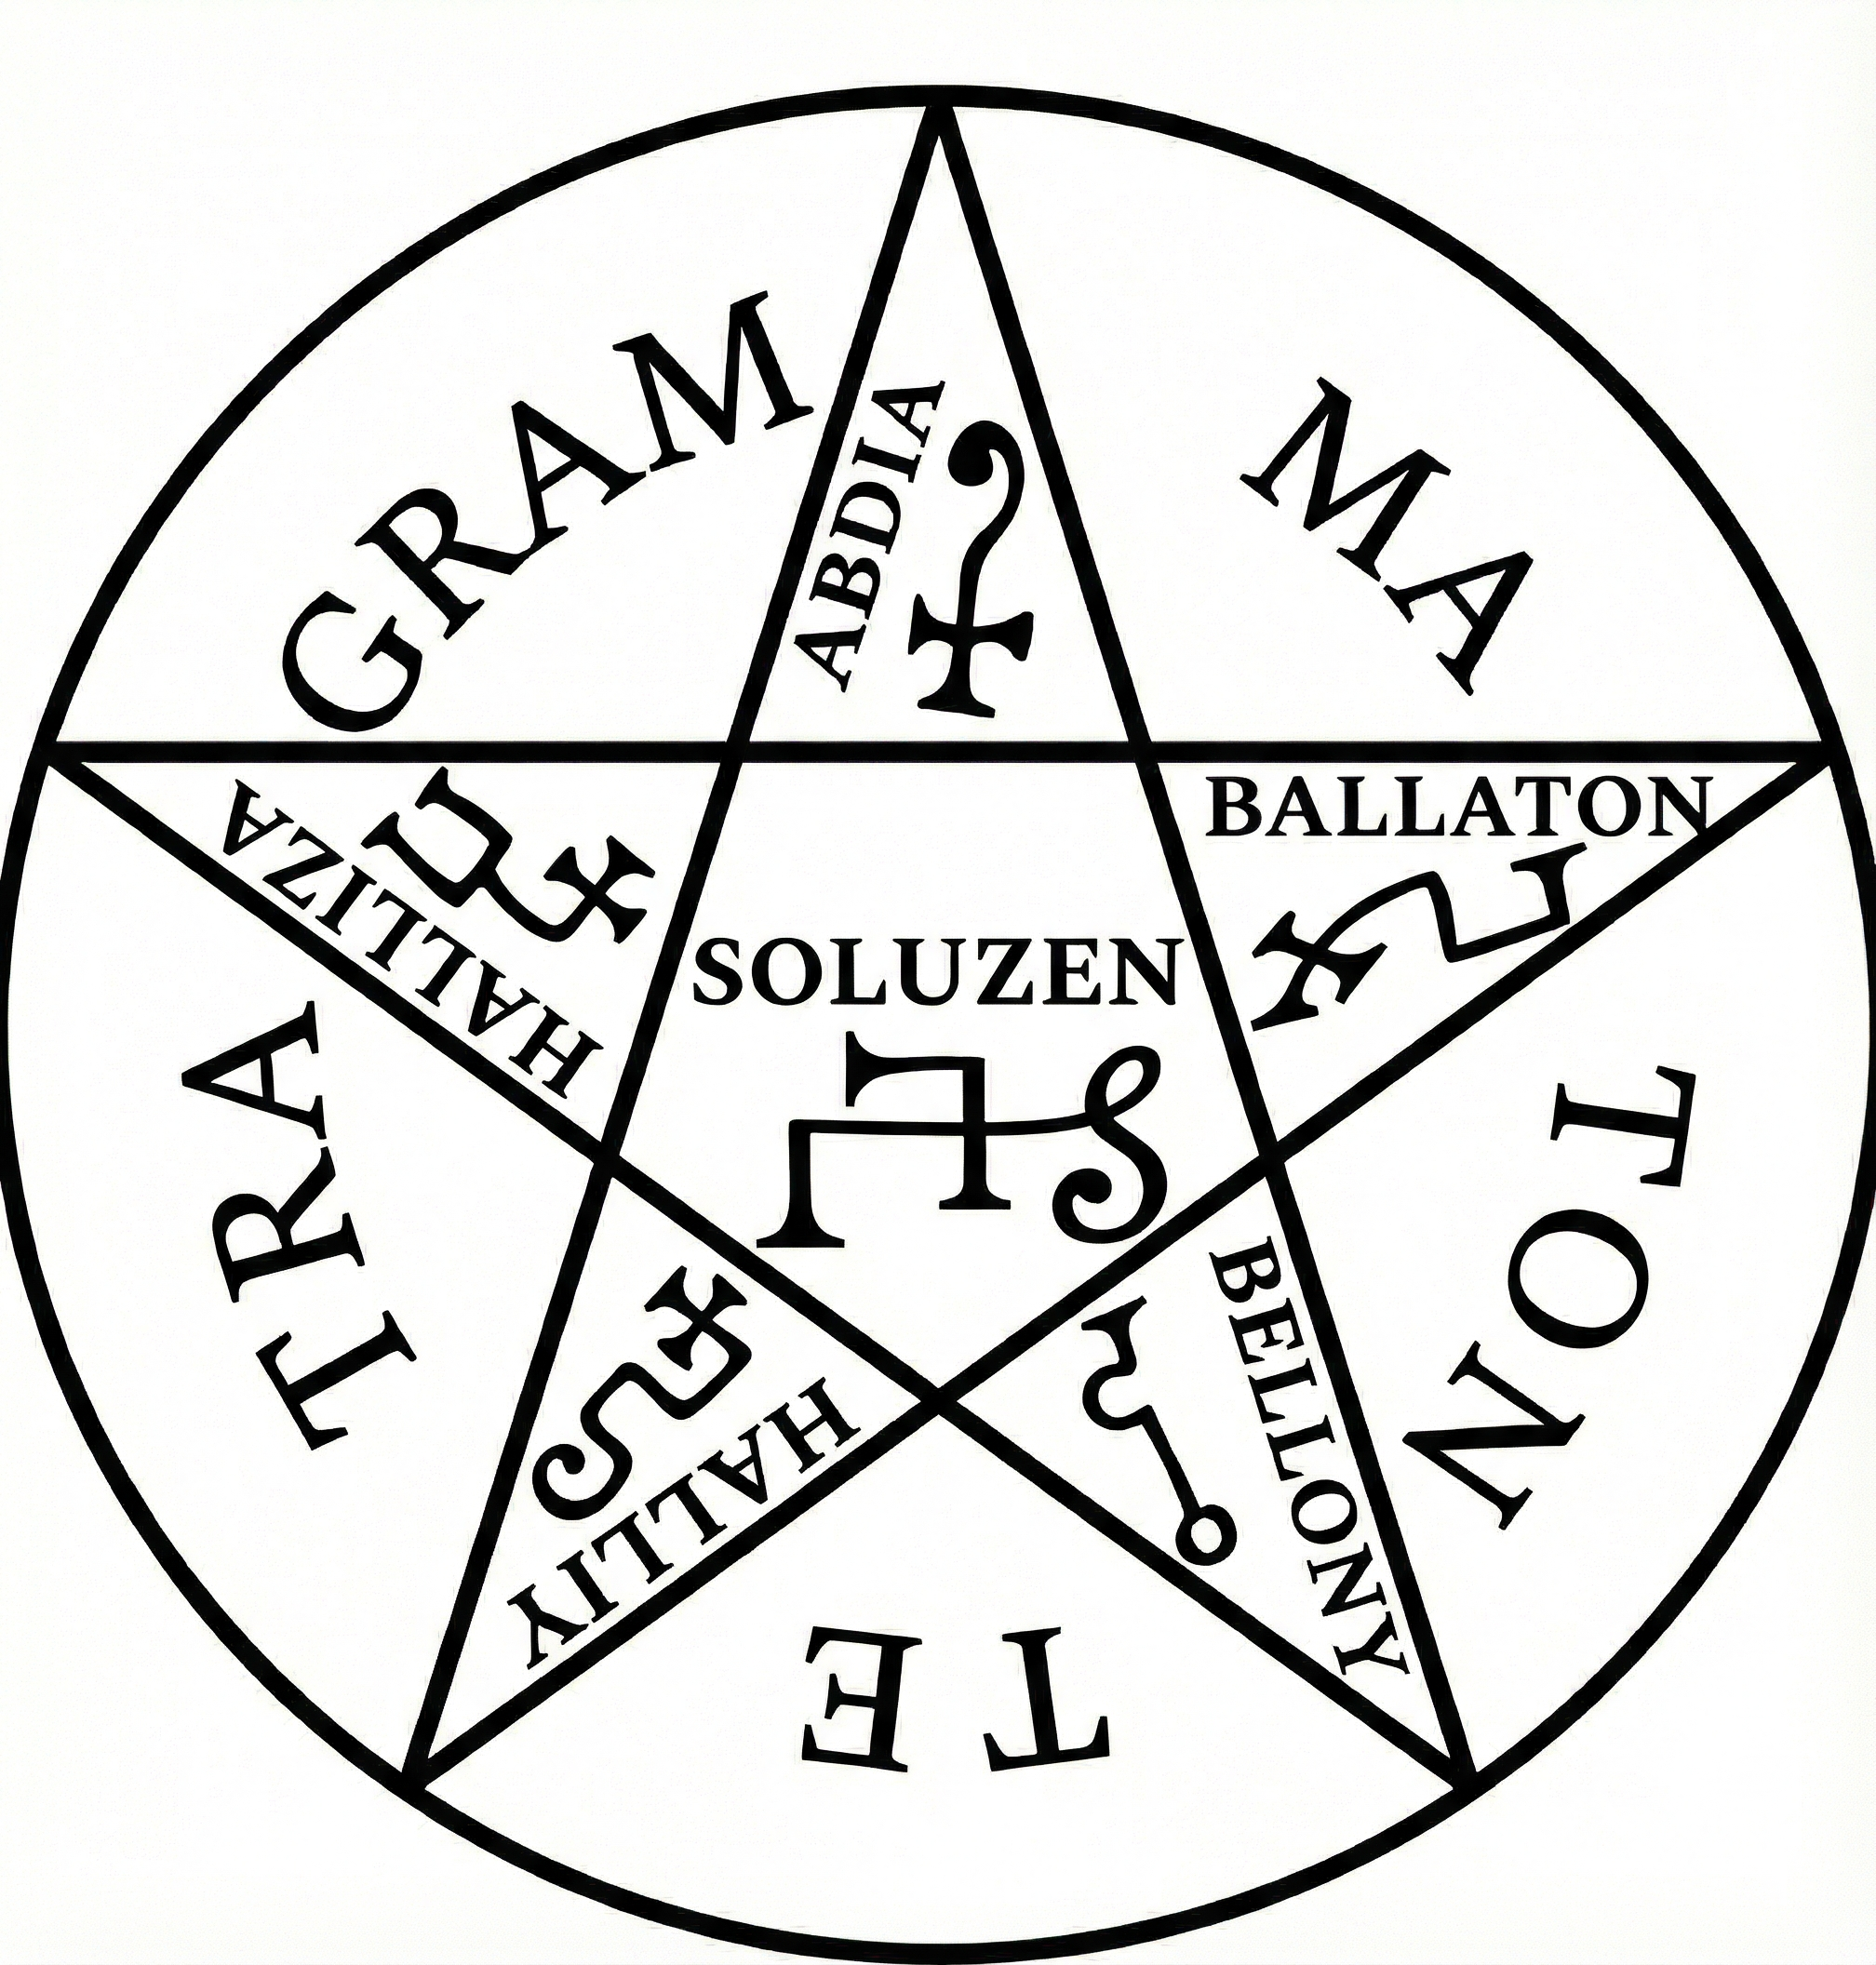
\includegraphics[width=0.3\paperwidth,keepaspectratio]{solomon_pentagram.png}
		\caption{The Pentagram of Solomon}
		\label{fig:solomonpentagram}
		\cite[39]{mathersgoetia1904}
	\end{figure}
	
	Elements:
	
	\begin{itemize}
		\item Five points: The five letters of YHShVH (Yahshuah---the {\textquotedblleft}pentagrammaton{\textquotedblright})
		\item Center: The letters TE-TRA-GRAM-MA-TON arranged in the inner pentagon
		\item Outer ring: ABDIA, BALLATON, BELLONY, HALLIY, HALLIZA, SOLUZEN
	\end{itemize}
	For generalized repulsion: Inscribe on metal (traditionally copper or silver). Wear or mount at thresholds.  The symbol asserts authority over any of the 72 without needing to know which.
	
	\subsection{Combined Form}
	\begin{figure}[H]
		\centering
		\includegraphics[width=0.3\paperwidth,keepaspectratio]{solomon_circle_and_triangle.png}
		\caption[Circle and Triangle]{Circle and Triangle\footnotemark}
		\label{fig:circletriangle}
	\end{figure}

	\footnotetext{Figures 153, 154 from de Laurence (Chicago, 1916)\cite{delaurence}, referenced but not included in Mathers (1904)\cite{mathersgoetia1904}.}

	\subsection{Spoken Formula for General Banishment}
	\begin{quotation}
	{\textquotedbl}By TETRAGRAMMATON, ADONAI, AGLA, ON, EL---depart from this place.  By PRIMEUMATON who commands thy
	beginning and ANAPHAXETON who binds thy form---return to the depths appointed unto thee.{\textquotedbl}
	\end{quotation}
	
	
	\bigskip
	
	\clearpage
	\section{ENTRAPMENT}
	\hspace{1cm}{\large Containing What Is Present and Localized}
	
	\subsection{The Triangle of Art (Trap Configuration)}
	For entrapment rather than repulsion, the triangle's point faces INWARD toward the disturbance.  This creates a snare
	that draws in and holds any intrusive entity.
	
	Place the triangle over the affected area (window, mirror, suspected portal). At each corner, drive an iron nail into
	the floor or ground.  Place a small pile of salt at each point.  Light black candles.
	
	Speak the Constraint:
	
	\begin{quotation}
	{\textquotedblleft}By PRIMEUMATON at the North, thy origin is sealed.  By ANAPHAXETON at the West, thy form is bound.  By TETRAGRAMMATON at the East, thy will is subject.  Within this triangle thou art constrained.  Thou canst not flee.  Thou canst not hide.  Thou must answer to the names of power.{\textquotedblright}		
	\end{quotation}
	
	\subsection{The Secret Seal of Solomon}
	This seal from the Goetia was used to constrain spirits inside a brass vessel.  It is already generalized---its power
	forces spirits to submit regardless of their rank or individual nature.
	
	The design:
	
	\begin{itemize}
		\item Concentric circles
		\item Central square containing divine names
		\item Hebrew letters around the perimeter
	\end{itemize}
	For defensive use:
	
	\begin{itemize}
		\item Place beneath the threshold of a space
		\item Inscribe on the lid of a container (to trap)
		\item Carve into a surface where an intrusion is suspected
	\end{itemize}
	\subsection{The Brass Vessel (Generalized Trap)}
	The original Goetia describes a brass vessel for containing spirits.  A generalized version:
	
	Construction:
	
	\begin{itemize}
		\item Brass body (copper + zinc alloy)
		\item Lead lid with Secret Seal of Solomon impressed
		\item Iron plate beneath
		\item Interior may contain: mercury in sealed glass, graveyard earth, salt, sulfur
	\end{itemize}
	
	\bigskip
	
	\clearpage
	\section{EXPULSION}
	\hspace{1cm}{\large Driving Out What Is Already Embedded}
	
	\subsection{Identifying the Attachment Type}
	Before expulsion, determine what the entity is attached to:
	
	\begin{flushleft}
		\begin{xltabular}{\textwidth}{|X|X|X|}
			\hline
			\textbf{Locational} & \textbf{Object-Bound} & \textbf{Personal} \\ \hline
			\endhead
			Activity in specific areas; doesn't follow people who leave &
			Disturbance centers on item; stops when item removed &
			Follows person; effects persist outside location \\ \hline
			Solution: Space cleansing and reconsecration &
			Solution: Destroy or seal the object &
			Solution: Personal severance ritual \\ \hline
			\caption{Attachment Type}
		\end{xltabular}
	\end{flushleft}
	\subsection{The Three Conjurations}
	The Goetic system escalates through increasingly severe conjurations.  Each level invokes higher powers and threatens
	greater consequences.
	
	\subsubsection{First Conjuration (Command)}
	\begin{quotation}
	{\textquotedblleft}I conjure and command thee, spirit present in this place, by the living God, by the true God, by the holy God, by the God who spoke and all was made, who commanded and all was created.  I conjure thee by TETRAGRAMMATON YHVH, who cast Adam from Eden, who brought the Flood upon the world, who consumed Sodom with fire, who parted the Red Sea.  I conjure thee by ADONAI, Lord of all creation, by EHYEH ASHER EHYEH, I Am That I Am, by EL SHADDAI, God Almighty, by ELOHIM GIBOR, God of Strength.  Thou art bound by these names.  Thou shalt not remain where thou art not welcome.  Thou shalt depart unto the place appointed thee.  By what name art thou called? By what authority didst thou enter? I command thee: SPEAK.{\textquotedblright}
	\end{quotation}
	
	\subsubsection{Second Conjuration (Threat)}
	\begin{quote}If resistance or silence, escalate:\end{quote}
	
	\begin{quotation}
	{\textquotedblleft}Spirit, thou hast not obeyed.  I conjure thee now by the dreadful Day of Judgment, by the Sea of Glass before the throne, by the Four Beasts with eyes before and behind, by the fire about the throne, by the holy angels of heaven, by the mighty wisdom of God.  I conjure thee by TETRAGRAMMATON YHVH, by ADONAI, EHYEH, EL, ELOHIM, by SADAY, ZEBAOTH, ELION, by ESCERCHIE, ORISTON, JAH, TETRAGRAMMATON.  If thou dost not obey, I will curse thee unto the depths of the abyss.  I will bind thee in chains of darkness.  I will trip from thee all rank and power.  DEPART.  NOW.  Unto the place from whence thou came.  Return not to this place, nor to any whom I protect.  By AGLA, be GONE.{\textquotedblright}
\end{quotation}
	
	\subsubsection{Third Conjuration (Curse)}
	\begin{quote}Final escalation with the four archangels:\end{quote}
	
	\begin{quotation}
	{\textquotedblleft}Disobedient and obstinate spirit, because thou hast not heeded the words of power, because thou hast defied the names of God, I curse thee in the name of TETRAGRAMMATON.  By ANAPHAXETON, I strip thy hidden protections.  By PRIMEUMATON, I sever thy connection to this place.  By TETRAGRAMMATON, I cast thee out utterly.  MICHAEL stands at the East with sword drawn.  GABRIEL stands at the West with the cup of banishment.  RAPHAEL stands at the South with the winds of driving.  URIEL stands at the North with flames of purification.  There is no quarter for thee.  There is no refuge.  I expel thee by the power of the Most High.  I expel thee by Solomon who bound thy kind.  I expel thee by the Seal that commands thy obedience.  GO.  TETRAGRAMMATON compels thee.  ADONAI compels thee.  AGLA compels thee.  EL.  YAH.  YHVH.  EHYEH.  SADAY.  BE GONE FROM THIS PLACE FOREVER.{\textquotedblright}
\end{quotation}
	
	\subsection{Severance Procedures}
	For Locational Attachment:
	
	\begin{enumerate}
		\item Take iron blade or nail
		\item Beginning at center of disturbance, {\textquotedblleft}cut{\textquotedblright} the air in a cross pattern
		\item Speak: {\textquotedblleft}I sever thy tie to this place.{\textquotedblright}
		\item Move to each corner of the room/space, repeat
		\item At threshold, cut horizontally across doorway: {\textquotedblleft}Thy passage here is ended.{\textquotedblright}
	\end{enumerate}
	For Object Attachment:
	
	Option A --- Destruction: Remove object to crossroads or running water.  Break it while speaking: {\textquotedblleft}By TETRAGRAMMATON, I break thy vessel.  By ADONAI, I release thy hold.  By AGLA, I end thy presence.{\textquotedblright} Bury fragments in separate locations or burn and scatter ashes in running water.
	
	Option B --- Sealing: Place in brass vessel with lead lid.  Seal with Secret Seal of Solomon.  Bind with iron chain or wire.  Bury deeply or encase in concrete.
	
	For Personal Attachment:
	
	\begin{enumerate}
		\item Person stands in center of Circle of Solomon
		\item Operator works from outside, with hazel wand
		\item Beginning at crown of head, move wand downward: {\textquotedblleft}From thy head, depart.{\textquotedblright}
		\item At throat: {\textquotedblleft}From thy voice, depart.{\textquotedblright}
		\item At heart: {\textquotedblleft}From thy heart, depart.{\textquotedblright}
		\item At hands: {\textquotedblleft}From thy works, depart.{\textquotedblright}
		\item At feet: {\textquotedblleft}From thy path, depart.{\textquotedblright}
		\item Final sweep, head to toe, with full severance declaration
		\item Person is anointed with protective oil and given Pentagram of Solomon to wear
	\end{enumerate}
	
	\bigskip
	
	\clearpage
	\section{THE FIFTY NAMES OF MARDUK}
	\hspace{1cm}{\large Babylonian Divine Authority for Exorcism}
	
	\subsection{Origin and Function}
	The Fifty Names of Marduk derive from the Babylonian creation epic, the {Enuma Elish}{\index{Enuma Elish}} (circa 12th century BCE). These names appear in Tablets VI and VII and represent powers given to Marduk after his victory over the chaos dragon Ti\={a}mat.
	
	These names were used in {\textquotedblleft}Marduk's Address to the Demons,{\textquotedblright} a key section of the ancient Mesopotamian exorcism series Udug-\d{h}ul ({\textquotedblleft}Evil Demons{\textquotedblright}). When performing exorcisms, the exorcist (\=a\v{s}ipu) would essentially become Marduk, speaking in the first person as Asallu\d{h}i/Marduk.
	
	The core principle: By reciting the Fifty Names, the exorcist assumes the identity and authority of Marduk himself---the god who defeated primordial chaos.
	
\subsection{The Fifty Names}
\begin{xltabular}{\textwidth}{|c|l|X|}
	\hline
	\textbf{\#} & \textbf{Name} & \textbf{Domain/Power} \\ \hline
	\endfirsthead
	\hline
	\textbf{\#} & \textbf{Name} & \textbf{Domain/Power} \\ \hline
	\endhead
	
	1 & \textsc{Marduk} & The Son of the Sun; he who establishes cosmic order. \\ \hline
	2 & \textsc{Marukka} & He who creates the wisdom of all. \\ \hline
	3 & \textsc{Marutukku} & Master of the arts of protection; hostile to the aggressor. \\ \hline
	4 & \textsc{Barashaku\v{s}u} & He who compelled the obedient into chaos; he who is wide of heart. \\ \hline
	5 & \textsc{Lugaldimmerankia} & Master of Order, who puts the wind demons to flight. \\ \hline
	6 & \textsc{Nari} & The Director, who regulates the heavens and earth. \\ \hline
	7 & \textsc{Asallu\d{h}i} & The Name of Power; the protector of the good, the banisher of the wicked. \\ \hline
	8 & \textsc{Namtila} & The Life-Giver; he who restores the dead to life. \\ \hline
	9 & \textsc{Namru} & The Bright One; he who purifies the path. \\ \hline
	10 & \textsc{Asaru} & Bestower of cultivation; who establishes the water levels. \\ \hline
	11 & \textsc{Asarualim} & He whose counsel is esteemed; the light of the gods. \\ \hline
	12 & \textsc{Asarualimnunna} & The Power that presides over the armor of the gods. \\ \hline
	13 & \textsc{Tutu} & He who silences the weeping; the supreme banisher. \\ \hline
	14 & \textsc{Ziukkina} & Life of the Host; he who establishes the heavens. \\ \hline
	15 & \textsc{Ziku} & The God of the Breath; Lord of Holiness. \\ \hline
	16 & \textsc{Agaku} & The Lord of the Charm; he who brings the dead to life. \\ \hline
	17 & \textsc{Tuku} & The Lord of the Ban; he whose spell is holy. \\ \hline
	18 & \textsc{\v{S}azu} & He who knows the heart; the searcher of souls. \\ \hline
	19 & \textsc{Zisi} & The Reconciler; the silencer of the enemy. \\ \hline
	20 & \textsc{Su\d{h}rim} & He who roots out the enemies with the weapon. \\ \hline
	21 & \textsc{Su\d{h}gurim} & He who destroys the foes; who makes the shell to vanish. \\ \hline
	22 & \textsc{Za\d{h}rim} & The Destroyer; he who grinds the enemy to dust. \\ \hline
	23 & \textsc{Za\d{h}gurim} & He who destroys the enemy in a specific way (the specialized destroyer). \\ \hline
	24 & \textsc{Enbilulu} & The Lord of the Abundance; he who governs the waters. \\ \hline
	25 & \textsc{Epadun} & The Lord of the Plain; who irrigates the fields. \\ \hline
	26 & \textsc{Gugal} & The Inspector of the Canals; the Lord of the Overflow. \\ \hline
	27 & \textsc{Hegal} & He who accumulates the harvest; who brings rain. \\ \hline
	28 & \textsc{Sirsir} & He who heaps up the mountain (of grain) upon the serpent. \\ \hline
	29 & \textsc{Mala\d{h}} & The Boatman; he who navigates the ship of state. \\ \hline
	30 & \textsc{Gil} & The Storehouse; the seed-preserver. \\ \hline
	31 & \textsc{Gilma} & The Founder; who renders the firmament permanent. \\ \hline
	32 & \textsc{Agilma} & The Lofty One; who removes the hoop (of constraint). \\ \hline
	33 & \textsc{Zulum} & The Divider; who assigns the fields. \\ \hline
	34 & \textsc{Mummu} & The Creator of the Universe; the One who was before. \\ \hline
	35 & \textsc{Zulummar} & The Hammer; he who crushes the opposition. \\ \hline
	36 & \textsc{Lugalabdubur} & The Destroyer of the Gods of Ti\={a}mat; the conqueror. \\ \hline
	37 & \textsc{Pagalguenna} & The Leader of all Lords; whose spirit is pre-eminent. \\ \hline
	38 & \textsc{Lugaldurma\d{h}} & The King of the Bond of the Gods; the Lord of the Link. \\ \hline
	39 & \textsc{Aranunna} & The Counselor of Ea; the creator of the treaty. \\ \hline
	40 & \textsc{Dumuduku} & The Son of the Holy Mound; the place of renewal. \\ \hline
	41 & \textsc{Lugalanna} & The King of the Height; the Lord of the Strength. \\ \hline
	42 & \textsc{Lugalugga} & The Lord of the Hosts of the Dead; he who extracts the life. \\ \hline
	43 & \textsc{Irkingu} & He who carried off the Kingu (Dragon-General) in the battle. \\ \hline
	44 & \textsc{Kinma} & The Judge and Governor of the Gods; the director of names. \\ \hline
	45 & \textsc{Esizkur} & He who sits in the House of Prayer; the hearer of vows. \\ \hline
	46 & \textsc{Gibi} & The One who maintains the Point; the creator of the winds. \\ \hline
	47 & \textsc{Addu} & The Storm King; who covers the sky with his shroud. \\ \hline
	48 & \textsc{A\v{s}aru} & The Overseer; who regulates the gods of destiny. \\ \hline
	49 & \textsc{Nebiru} & The Star of the Pole; he who holds the pivot of the stars. \\ \hline
	50 & \textsc{Nibbura} & Father Enlil bestowed this name: The Lord of the Lands. \\ \hline
	\caption[The Fifty Names of Marduk]{The Fifty Names of Marduk \\ \cite{speiser1969}}
	\end{xltabular}
	
	\subsection{Using the Names in Exorcism}
	The exorcist declares each name in the first person, assuming Marduk's identity:
	
	{\textquotedblleft}I am Asallu\d{h}i, magician of the gods.  I am MARDUK, supreme authority.  I am ASARULUDU, wielder of the flaming sword.  I am NAM\-TIL\-LA\-KU, who speaks with spirits.  I am LUG\-GAL\-DIM\-MER\-ANK\-IA, who commands the wind demons and puts order into chaos.  By these names, I command thee: DEPART.{\textquotedblright}
	
	
	\bigskip
	
	\clearpage
	\section{ROMAN CATHOLIC FORMULAS}
	\hspace{1cm}{\large Traditional Christian Exorcism Prayers}
	
	\subsection{The Vade Retro Satana}
	This medieval Western Christian formula for exorcism was recorded in a 1415 manuscript found in the Benedictine {Metten Abbey}{\index{Metten Abbey}} in Bavaria.  It received the approval of {Pope Benedict XIV}{\index{Pope Benedict XIV}} in 1742 and became part of the Roman Catholic ritual.  The initials are engraved on the Saint Benedict Medal.
	
	\begin{xltabular}{\textwidth}{|X|X|}
		\hline
		\textbf{Latin} & \textbf{English} \\ \hline
		\endhead
		\hline

		Crux sacra sit mihi lux.  Non draco sit mihi dux Vade retro satana Numquam suade mihi vana.  Sunt mala quae libas.  Ipse venena bibas
		&	
		May the holy cross be my light.  May the dragon never be my guide Begone, Satan! Never tempt me with your vanities.  What you offer is evil.  Drink the poison yourself! \\ \hline
		\caption{Vade Retro Satana}
	\end{xltabular}
	
	\subsection{Prayer to Saint Michael the Archangel}
	Introduced by {Pope Leo XIII}{\index{Pope Leo XIII}} in 1886 following his reported vision of demonic spirits.  The short form was mandated to be prayed after every Low Mass until 1964.
	
	Short Form:
	
	\begin{xltabular}{\textwidth}{|X|X|}
		\hline
		\textbf{Latin} & \textbf{English} \\
		\hline
		\endhead
		\hline
		Sancte Michael Archangele, defende nos in proelio; contra nequitiam et insidias diaboli esto praesidium.  Imperet illi Deus, supplices deprecamur: tuque, Princeps militiae caelestis, Satanam aliosque spiritus malignos, qui ad perditionem animarum pervagantur in mundo, divina virtute in infernum detrude.  Amen.
		&
		Saint Michael the Archangel, defend us in battle; be our protection against the wickedness and snares of the devil.  May God rebuke him, we humbly pray:and do thou, O Prince of the heavenly host, by the power of God, thrust into Hell Satan and all the other evil spirits who prowl about the world seeking the ruin of souls.  Amen. \\
		\hline
		\caption{Prayer to Saint Michael the Archangel}
	\end{xltabular}
	
	\subsection{The Exorcismus in Satanam et Angelos Apostaticos}
	The long form exorcism prayer composed by {Pope Leo XIII}{\index{Pope Leo XIII}} in 1890, incorporated into the Roman Ritual in 1898.  This is reserved for use by bishops and authorized priests.  As found in the traditional rite \cite{leo1890exorcism}, the invocation begins with “In nómine Iesu Christi…”\\
	Key Passages:
	\vspace{1.0cm}
	\begin{quotation}
		{\textquotedblleft}In the Name of Jesus Christ, our God and Lord,\\strengthened by the intercession of the Immaculate Virgin Mary, Mother of God,\\of Blessed Michael the Archangel,\\of the Blessed Apostles Peter and Paul and all the Saints,\\and powerful in the holy authority of our ministry,\\we confidently undertake to repulse the attacks and deceits of the devil...{\textquotedblright}

		{\textquotedblleft}God arises;\\His enemies are scattered\\and those who hate Him flee before Him.\\As smoke is driven away, so are they driven;\\as wax melts before the fire, so the wicked perish at the presence of God...{\textquotedblright}
	
		{\textquotedblleft}God the Father commands you.\\God the Son commands you.\\God the Holy Ghost commands you.\\Christ, God's Word made flesh, commands you.\\The glorious Mother of God, the Virgin Mary, commands you.\\The faith of the holy Apostles Peter and Paul, and of the other Apostles commands you.\\The blood of the Martyrs and the pious intercession of all the Saints command you.{\textquotedblright}
	\end{quotation}
	\vspace{0.5in}
	\begin{quotation}
		In nómine Iesu Christi, Dei et Dómini nostri, \\
		intercessióne Immaculátæ Vírginis Dei Genetrícis Maríæ, \\
		Beáti Michaélis Archángeli, Beáti Ioánnis Baptístæ, \\
		Sanctórum Apostolórum Petri et Páuli et ómnium Sanctórum, \\
		fidúcia ministérii nostri sacri, \\
		adversus versútias et insídias diáboli cum fidúcia aggredímur. \\[1ex]
		
		Exsúrgat Deus, et dissipéntur inimíci eius: \\
		et fúgiant qui odérunt eum a fácie eius. \\
		Sicut déficit fumus defíciant; \\
		sicut fluit cera a fácie ígnis, \\
		sic péreant peccatóres a fácie Dei. \\[1ex]
		
		Imperat tibi Deus Pater, \\
		imperat tibi Deus Fílius, \\
		imperat tibi Deus Spíritus Sanctus. \\
		Imperat tibi Maiéstas Christi, Verbum Dei incarnátum. \\
		Imperat tibi Virgo gloriósa, Dei Genetrix María. \\
		Imperat tibi fides Sanctórum Apostolórum Petri et Páuli \\
		et aliórum Apostolórum. \\
		Imperat tibi sanguis Mártyrum, \\
		imperat tibi pia intercessió Sanctorum et Sanctárum. \\
	\end{quotation}
	
	\bigskip
	
	\clearpage
	\appendix
	\setcounter{table}{0}
	\renewcommand{\thetable}{A.\arabic{table}} % appendix-style numbering
	\clearpage
	\section{PRONUNCIATION GUIDE}
	\subsection{Sumero-Akkadian Phonetics}
	The following diacritical marks are used in the transcription of the Fifty Names to ensure correct pronunciation of the divine vibrations.
	
	\begin{xltabular}{\textwidth}{|c|l|X|}
		\hline
		\textbf{Symbol} & \textbf{Sound} & \textbf{Example} \\ \hline
		\endhead
		\v{s} & \textbf{sh} as in \textit{ship} & \textsc{\v{S}azu} (pronounced \textit{Shah-zoo}) \\ \hline
		\d{h} & \textbf{ch} as in Scottish \textit{loch} & \textsc{Asallu\d{h}i} (pronounced \textit{Ah-sall-oo-khee}) \\ \hline
		\d{t} & Emphatic \textbf{t}, hard stop & \textit{\d{T}uppu} (Tablet) \\ \hline		\d{s} & Emphatic \textbf{s} (ts sound) & \textit{Mu\d{s}a\d{s}ir} \\ \hline
		\={a}, \={e}, \={u} & Long vowels, held for double duration & \textit{E\={n}\={u}ma Eli\v{s}} \\ \hline
	\end{xltabular}
	\section{MATERIALS AND TIMING}
	\subsection{Metals and Their Uses}

	\begin{table}[h]
		\caption{Metals and Their Uses}
		\label{tab:metals}
		\begin{xltabular}{\textwidth}{|X|X|X|X|}
			\hline
			\textbf{Metal} & \textbf{Planet} & \textbf{Property} & \textbf{Use in Defense} \\ \hline
			\endhead
			Lead   & Saturn & Restriction, binding  & Trapping seals, vessel lids \\ \hline
			Iron   & Mars   & Aggression, repulsion  & Threshold nails, blades     \\ \hline
			Silver & Moon   & Reflection, purity     & Pentagram pendants          \\ \hline
			Copper & Venus  & Conductivity, harmony  & Circle inscriptions         \\ \hline
			Brass  & ---    & Containment            & Binding vessels             \\ 		\hline
		\end{xltabular}
	\end{table}
	\subsection{Incenses}
\begin{table}[h]
	\setcounter{table}{1}
	\caption{Incenses}
	\label{tab:incenses}
	\begin{xltabular}{\textwidth}{|l|X|}
		\hline
		\textbf{Purpose} & \textbf{Incense} \\ \hline
		\endhead
		Purification & Frankincense \\ \hline
		Authority/Command & Frankincense + mastic \\ \hline
		Repulsion & Asafoetida, sulfur, black pepper \\ \hline
		Binding & Myrrh + sulfur \\ \hline
		Sealing & Benzoin \\ \hline
	\end{xltabular}
\end{table}
	\subsection{Timing}
	Optimal conditions for defensive work:
	
	\begin{itemize}
		\item Moon phase: Waning (for banishing/repulsion) or Dark (for binding/trapping)
		\item Day: Saturday (Saturn---binding, endings) or Tuesday (Mars---aggressive action)
		\item Hour: Saturn hour for binding; Mars hour for repulsion; Sun hour for authority
		\item Moon sign: Earth signs (Taurus, Virgo, Capricorn) for permanence
	\end{itemize}
	
	\bigskip
	
	\clearpage

	\section{QUICK REFERENCE PROCEDURE}
	\subsection{Complete Procedure Checklist}
	PREPARATION
	
	\begin{enumerate}
		\item Timing: Waning/dark moon, Saturday/Tuesday, Saturn/Mars hour
		\item Personal cleansing and protection (salt bath, white garment, Pentagram)
		\item Circle of Solomon established
		\item Materials gathered: hazel wand, iron blade/nails, salt, holy water, incenses, candles
	\end{enumerate}
	CONSTRAINT
	
	\begin{enumerate}
		\item Triangle of Art placed over affected area
		\item Iron nails at corners
		\item Black candles lit
		\item Constraint formula spoken
	\end{enumerate}
	EXPULSION
	
	\begin{enumerate}
		\item First Conjuration (command)
		\item Second Conjuration (threat) --- if needed
		\item Third Conjuration (curse) --- if needed
		\item Physical severance with iron
		\item Recitation of Marduk names (optional layer)
		\item Vade Retro Satana / St.  Michael prayer (optional layer)
	\end{enumerate}
	CLEANSING
	
	\begin{itemize}
		\item Purification incense (frankincense, benzoin, camphor)
		\item Salt water throughout
		\item All corners and thresholds addressed
	\end{itemize}
	RECONSECRATION
	
	\begin{itemize}
		\item White candle circuit (clockwise)
		\item Hexagram placed at center
		\item Quarters sealed with pentagrams
		\item Protective installations in place
	\end{itemize}
	\subsection[Emergency Short{}-Form Procedure]{Emergency Short-Form Procedure}
	When full ritual isn't possible:
	
	\begin{itemize}
		\item Hold iron object (nail, blade, key)
		\item Speak firmly: {\textquotedblleft}By TETRAGRAMMATON, thou art commanded.  By ADONAI, thou art expelled.  By AGLA, thou art barred from return.  DEPART NOW.{\textquotedblright}
		\item Cast salt toward disturbance
		\item Trace pentagram in air, speak {\textquotedblleft}AGLA{\textquotedblright} as you complete it
		\item Repeat as needed, increasing intensity
		\item Add: {\textquotedblleft}Vade retro satana!{\textquotedblright} and/or St.  Michael prayer
	\end{itemize}
	
	\bigskip
	\clearpage
	\addtocontents{lof}{\protect\addvspace{10pt}}
	\addtocontents{lof}{\protect\contentsline{figure}{\textbf{Full Size Figures}}{}{}}
	
	
	\section{Full Size Images}
	\begin{figure}[p]
		\centering
		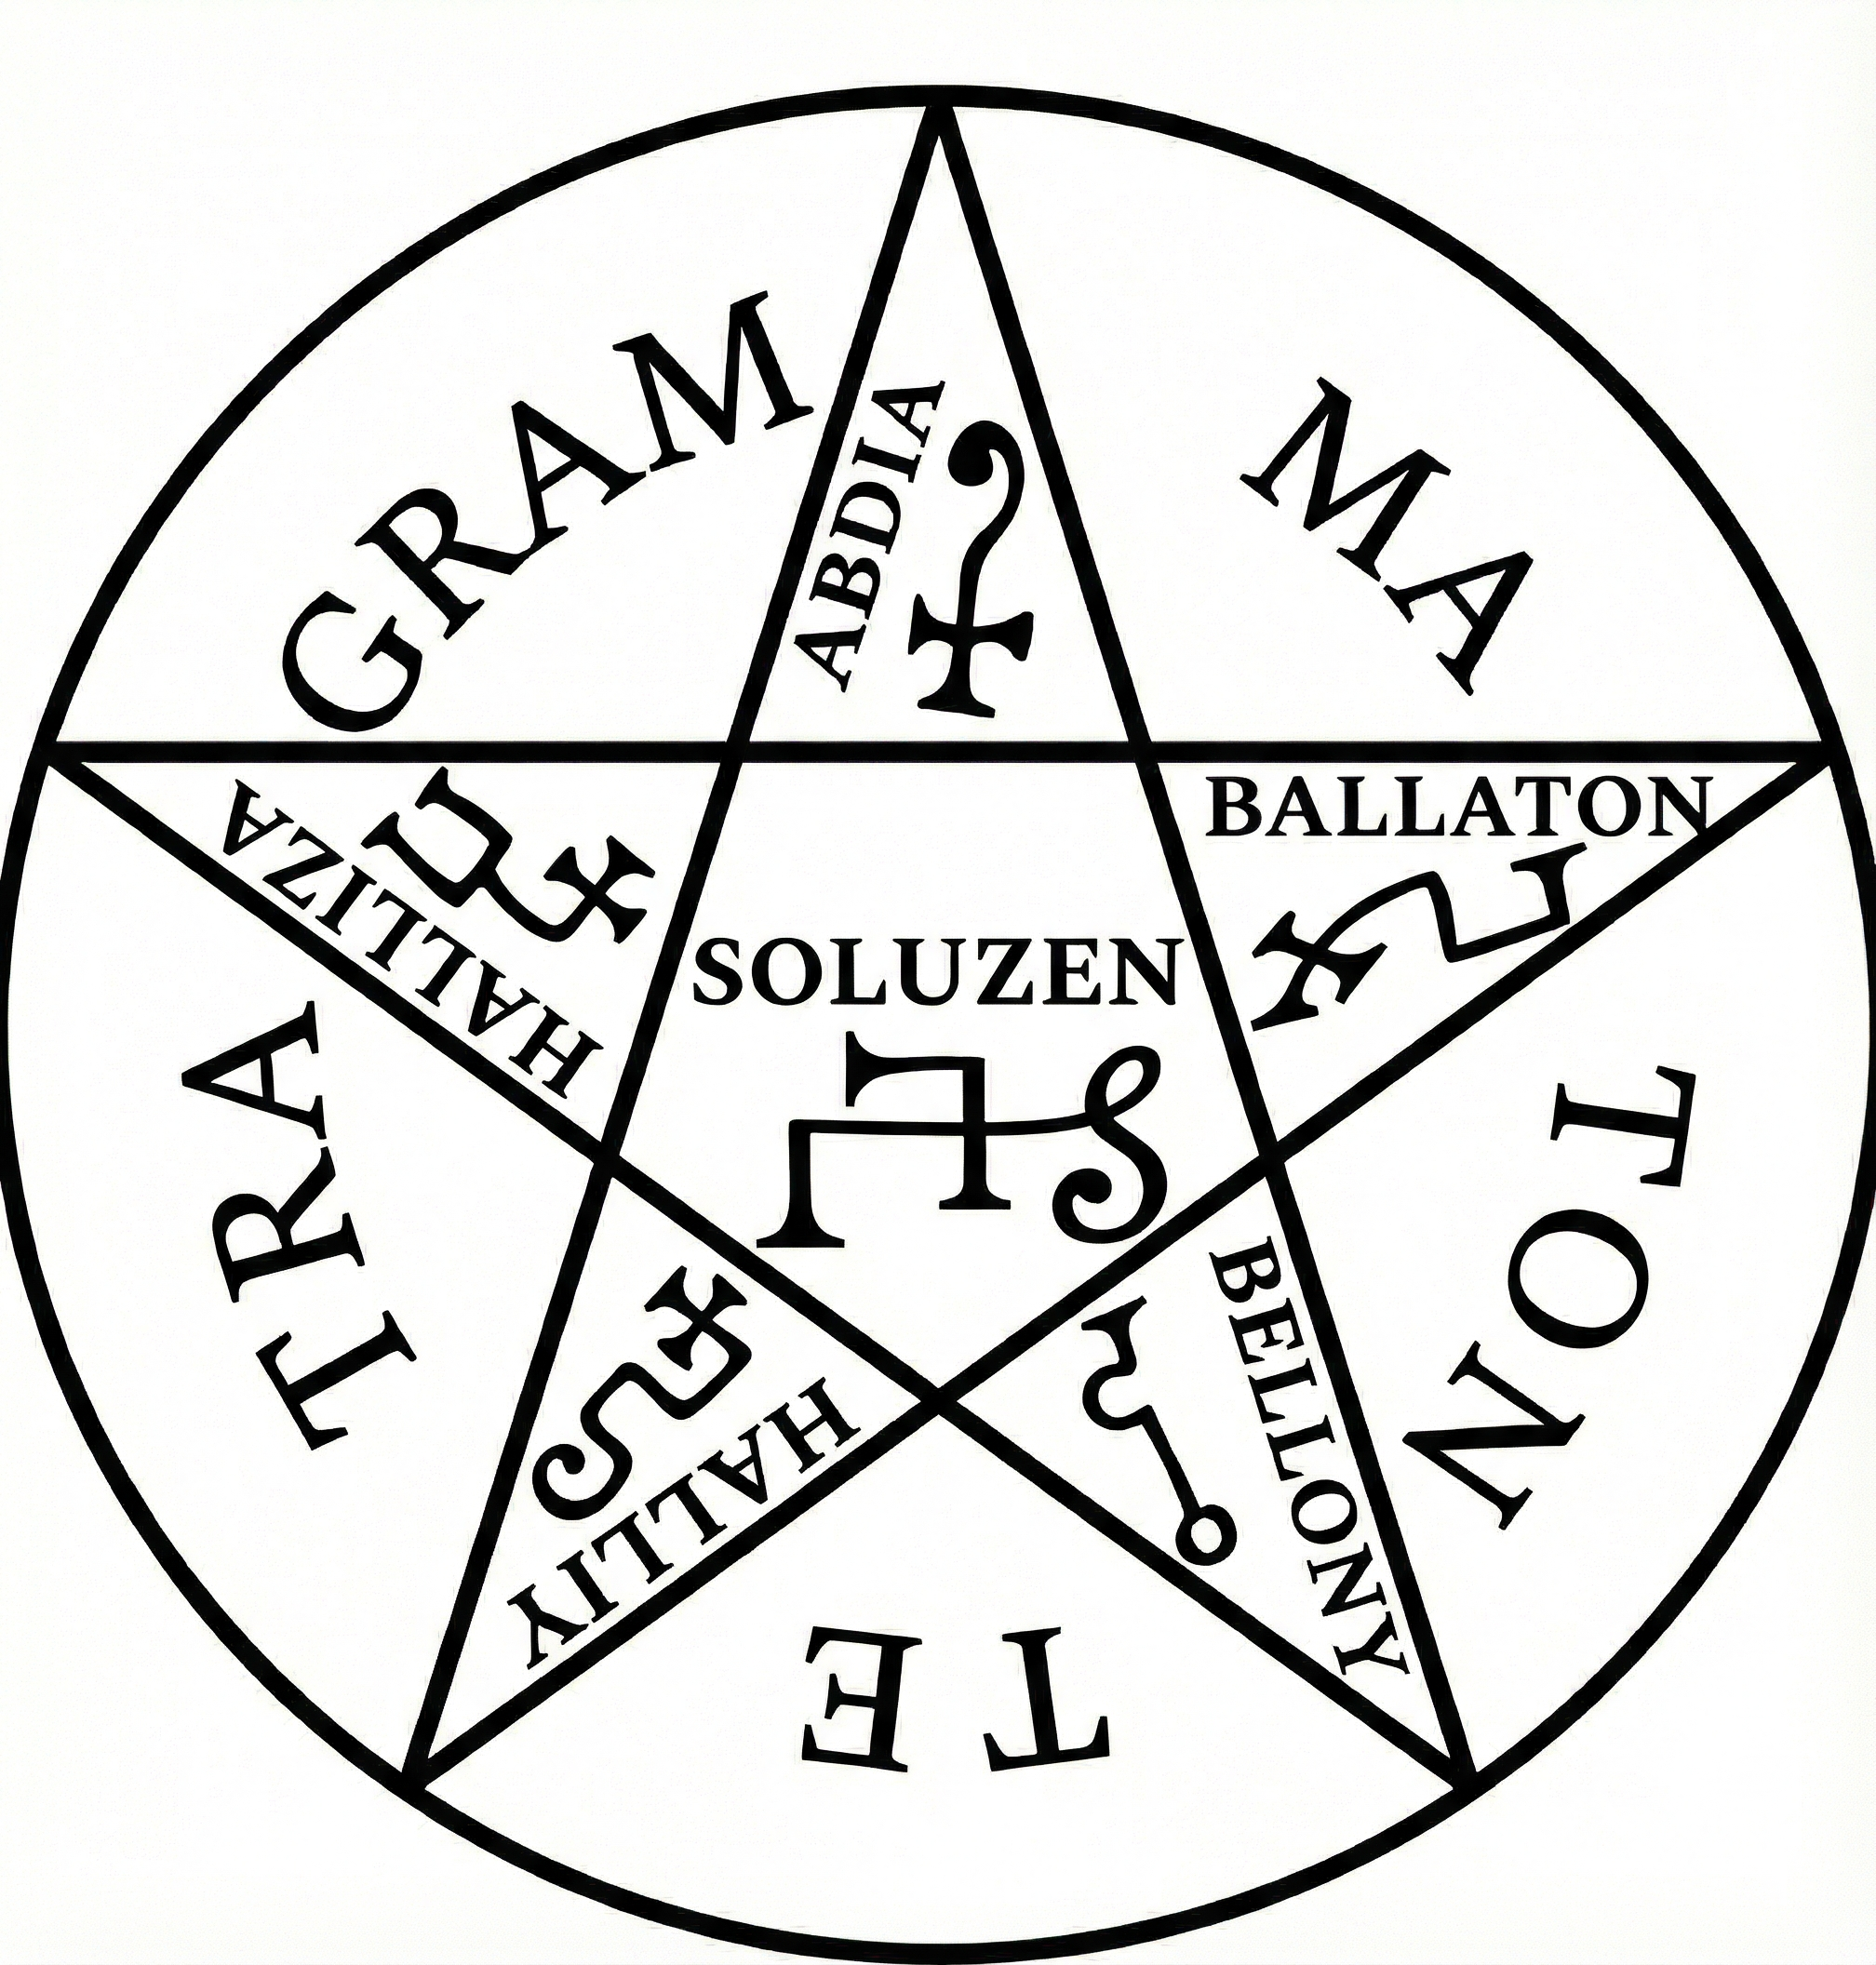
\includegraphics[width=0.8\paperwidth,keepaspectratio]{solomon_pentagram.png}
		\caption{The Pentagram of Solomon}
		\label{fig:solomonpentagramfull}
	\end{figure}
	\clearpage
	\begin{figure}[p]
	\centering
	\includegraphics[width=0.8\paperwidth,keepaspectratio]{solomon_hexagram.png}
	\caption{The Hexagram of Solomon}
	\label{fig:solomonhexagramfull}
\end{figure}
\clearpage
	\begin{figure}[p]
	\centering
	\includegraphics[width=0.8\paperwidth,keepaspectratio]{solomon_triangle.png}
	\caption{The Triangle of Art}
	\label{fig:solomontrianglefull}
\end{figure}
\clearpage
	\begin{figure}[p]
	\centering
	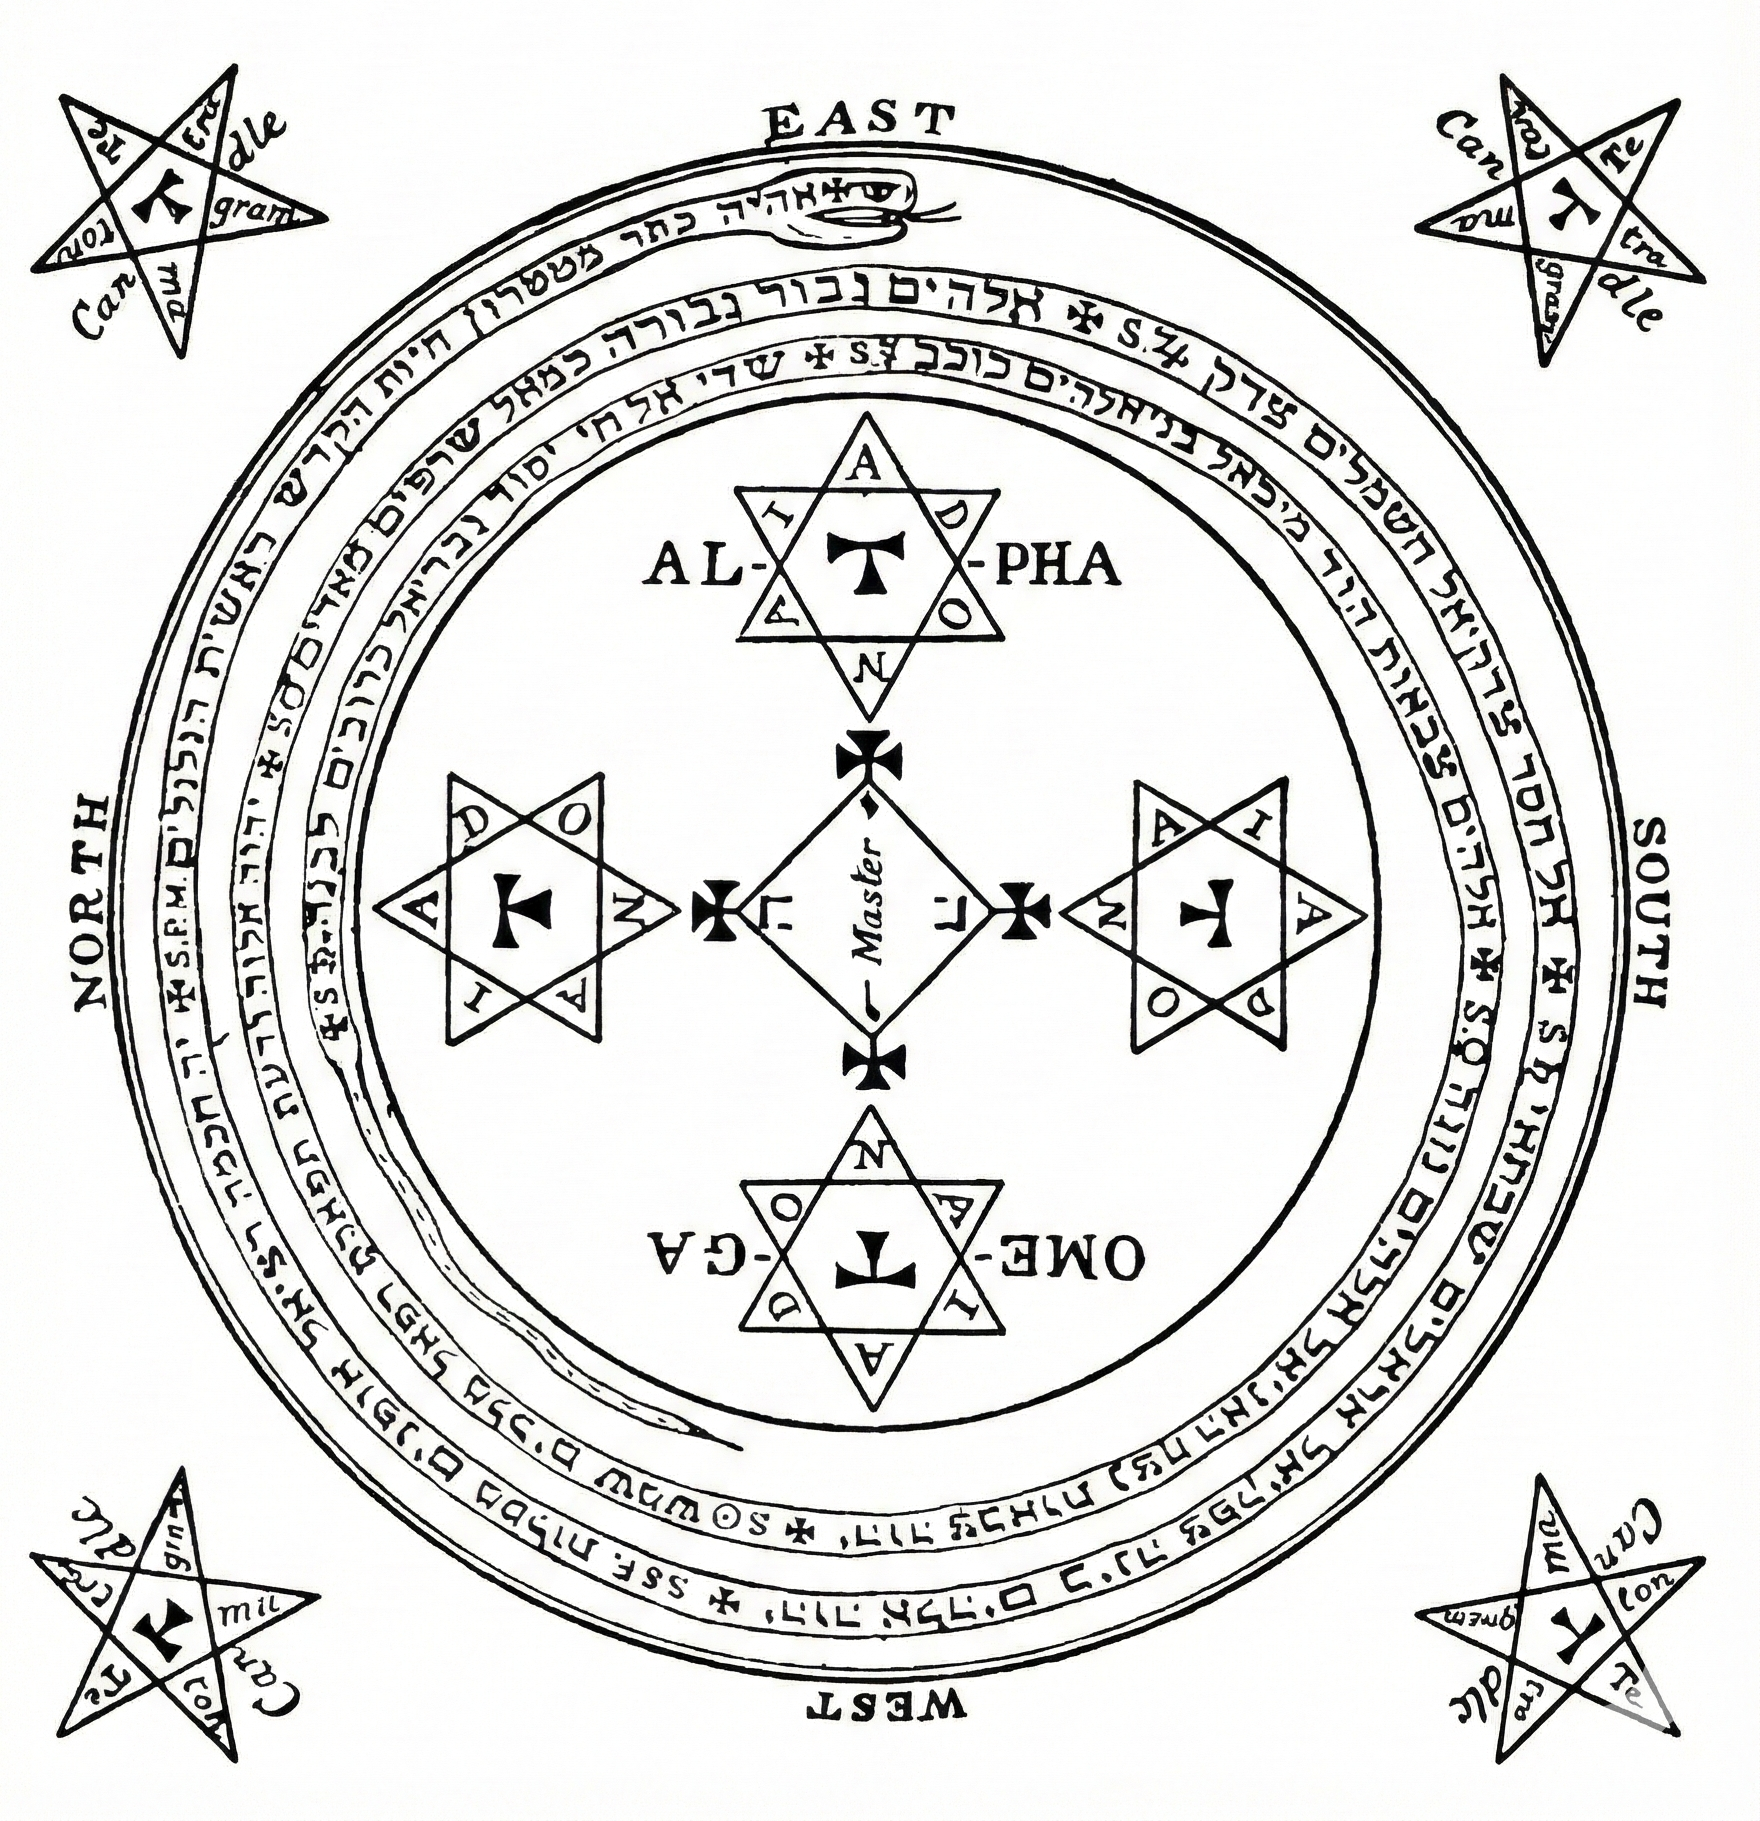
\includegraphics[width=0.8\paperwidth,keepaspectratio]{solomon_circle.png}
	\caption{The Circle of Solomon}
	\label{fig:solomoncirclefull}
\end{figure}
\clearpage
	\begin{figure}[p]
	\centering
	\includegraphics[width=0.8\paperwidth,keepaspectratio]{solomon_circle_and_triangle.png}
	\caption{Frontispiece}
	\label{fig:solomonfront}
\end{figure}
\clearpage
	\begin{center}
		{\Large FINIS}	\\
		\bigskip
		\textsl{	By the authority of the divine names, may this work serve those who seek protection.
		}	\\
		\bigskip
		TETRAGRAMMATON \textbullet{} ADONAI \textbullet{} AGLA \textbullet{} MARDUK \textbullet{} MICHAEL
	\end{center}
	\clearpage
	\printbibliography[keyword=babylonian,title={Sources for Babylonian Rituals}]
	\printbibliography[keyword=catholic,title={Sources for Catholic Liturgical Texts}]
	\printbibliography[keyword=occult,title={Sources for Occult Literature}]
	\clearpage
	\printglossaries
	\clearpage
	\printindex
\end{document}